\setcounter{chapter}{4}
\chapter{Alteration made in the Oslo CTM3}\label{chap:CTM3_Setup}

This chapter describes the setup and altered modules of the Oslo CTM3. 

\section{Setup of The Model}

A degraded resolution was used for the runs in the CTM3. In the \texttt{Makefile} it is possible to degrade the horizontal resolution by combining several boxes into one. The setting used for running the model was \texttt{HWINDOW=HFOUR}, i.e. a combination of four native boxes and thus a $4.5^o \times 4.5^o$ resolution (Illustrated in Figure \ref{fig:res_map}). In the vertical, 60 layers were used. The setup of the \texttt{Makefile} is explained more in Appendix \ref{subsubsec:makefile}. 

\medskip

The stratosphere was turned off in all the branches in order to save CPU time and to avoid conflict with the organic bromide sources (see Section \ref{sec:oceanic_emissions}). How this was performed is explained in Appendix \ref{app:turning_off_the_stratosphere}. 

\begin{figure}[ht]
    \centering
    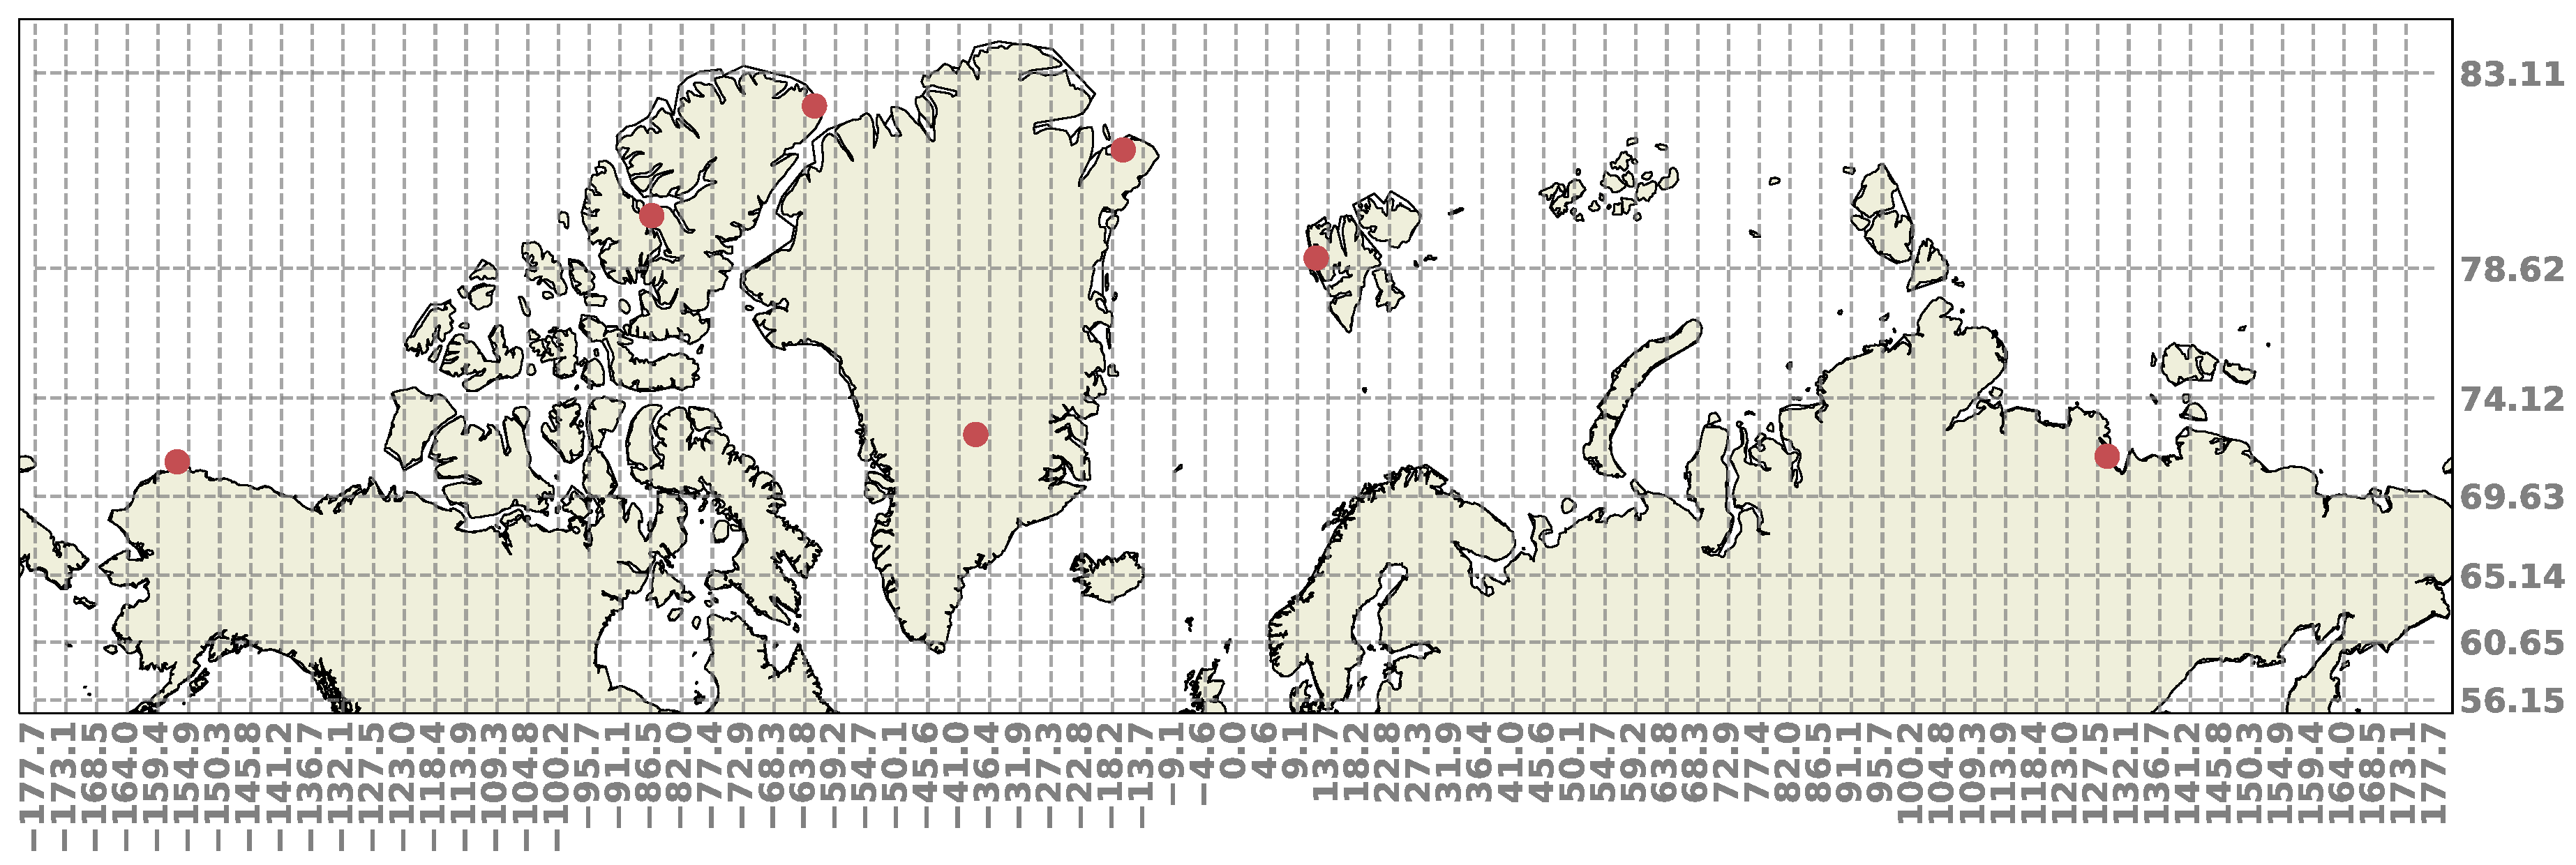
\includegraphics[width = \linewidth]{Chapter5_CTM3setup/images/resolution_map_Arctic.pdf}
    \caption{Illustration of the grid coverage in the Arctic at \texttt{HFOUR} $=$ 4.5$^o$x4.5$^o$ resolution. The red dots are the stations that were used for observational data}
    \label{fig:res_map}
\end{figure}


\medskip

To run the CTM3, a supercomputer is required. At the beginning of my master thesis the supercomputer Abel (\cite{abel}) was used. In January 2020, Abel was shut down and the Oslo CTM3 migrated to Saga (\cite{saga}). There are some differences between the two  and these differences as well as the setup of the model runs are explained in Appendix \ref{app:supercomputer}. 


\section{Wet deposition - \texttt{scavenging\_wet.inp}}\label{sec:scav_wet}

Wet scavenging rates for \chem{HCl}, \chem{HBr} and $\chem{ClONO_2}$ were added to the wet deposition input table \texttt{scavenging\_wet.inp}. The Henry's law constants are listed in Table \ref{tab:Henrys_law} and the wet deposition and Henry's law is explained in Section \ref{sec:wet_dep_henrys_law}. 

\begin{table}[ht]
\begin{tabular}{|lllll|}
\hline
\textbf{Component}          & \textbf{H$^{cp}$ [mol m$^{-3}$Pa]} & \textbf{$\frac{d \ln H^{cp}}{d(1/T)}$ [K]} & \textbf{Note} & \textbf{Reference}                \\ \hline
\chem{HCl} & $1.1\times10^{-2}$                     & $2300$                                         & (*)          & \cite{MARSH1985} \\
\chem{HBr} & $2.4\times10^{-1}$                     & $370$                                          & (**)         & \cite{dean1999}  \\
$\chem{ClONO_2}$            &  $2.1\times10^{5}$.   & $8700$                              & (***)       & \cite{Lelieveld1991TheRO}      \\ \hline
\end{tabular}
\caption{The Henry's law constants are taken from \cite{Sander2015} and references therein. 
\\
(*) Thermodynamical calculation  
\\ 
(**) Only the tabulated data between T = 273 K and T = 303 K from Dean (1992) were used to derive H and its temperature dependence. Above T = 303 K, the tabulated data could not be parameterized very well. The partial pressure of water vapor (needed to convert some Henry's law constants) was calculated using the formula given by Sander et al. (1995). The quantities A and $\alpha$ from Dean (1992) were assumed to be identical. 
\\ 
(***) Assumed to have the same Henry's law as $\chem{HNO_3}$ \cite{TerjePersonal}
\\
\textbf{Note: the units of the Henry's law constants were changed after this implementation (see the Results Section \ref{sec:res_step3}. It was changed to atm M$^{-1}$}}
\label{tab:Henrys_law}
\end{table}

 


\section{Implementation of halogen chemistry}

In essence, three modules were changed to implement the halogen chemistry. They were \texttt{pchemc\_ij.f90}, \texttt{tropchem\_oslo.f90} and \texttt{chem\_oslo\_rates.f90}. The base for the scripting is the work performed by \cite{Susanne}, which I have continued to alter.  The reactions that were implemented in the various modules can be seen in Table \ref{tab:3}.


%Some of the problems that occurred during this process, how these were tested and attemptedly solved, can be seen in Section \ref{chap:problem_solving}.
\begin{table}[ht]
\centering
\resizebox{12cm}{!}{%
\begin{tabular}{|l|l|l|}
\hline
\multicolumn{1}{|l|}{\textbf{Variable name CTM3}} & \multicolumn{1}{l|}{\textbf{Reaction}}                                                    & \textbf{Reaction no.}      \\ \hline
%\texttt{hobr\_dep}               & $\chem{HOBr} + \chem{HBr} \xrightarrow{aerosol} \chem{Br_2} + \chem{H_2O}$                & \ref{R:8} \\
\texttt{hobr\_dep}               & $\chem{HOBr} + \chem{H^+} + \chem{Br^-} \xrightarrow{snow/ice} \chem{Br_2} +\chem{H_2O} $ & \ref{R:7} \\
%\texttt{hobr\_dep}               & $\chem{HOBr} + \chem{HCl} \xrightarrow{aerosol} \chem{BrCl} + \chem{H_2O} $               & \ref{R:8} \\
\texttt{hobr\_dep}               & $\chem{HOBr} + \chem{H^+} + \chem{Cl^-} \xrightarrow{snow/ice} \chem{BrCl} +\chem{H_2O} $ & \ref{R:7} \\
\texttt{no2\_bro}                & $\chem{BrO} + \chem{NO_2} + M \rightarrow \chem{BrONO_2} + M$                             & \ref{R:9} \\
\texttt{oh\_chbr3}               & $\chem{CHBr_3} + \chem{OH} \rightarrow 3\chem{Br} + \chem{Products}$                      & \ref{R:10} \\
\texttt{oh\_chbr3}               & $\chem{CH_2Br_2} + \chem{OH} \rightarrow 2\chem{Br} + \chem{Products}$                    & \ref{R:11} \\
%\texttt{DCH\_3Br}                & $\chem{CHBr_3} + hv \rightarrow 3\chem{Br} + \chem{Products}$                             & \ref{R:12} \\ 
\texttt{brono2\_h2o}             & $\chem{BrONO_2} + \chem{H_2O} \xrightarrow{aerosol} \chem{HOBr} + \chem{HNO_3}$           & \ref{R:13}\\
\texttt{hobr\_hcl}               & $\chem{HOBr} + \chem{HCl} \xrightarrow{aerosol} \chem{BrCl} + \chem{H_2O}$                & \ref{R:8} \\
\texttt{hobr\_hbr}               & $\chem{HOBr} + \chem{HBr} \xrightarrow{aerosol} \chem{Br_2} + \chem{H_2O}$                & \ref{R:8} \\
\texttt{o3\_cl}                  & $\chem{O_3} + \chem{Cl} \rightarrow \chem{ClO} + \chem{O_2}$                              & \ref{R:2} \\
\texttt{no\_bro}                 & $\chem{BrO} + \chem{NO} \rightarrow \chem{NO_2} + \chem{Br}$                              & \ref{R:14} \\
\texttt{oh\_clo\_a}              & $\chem{OH} + \chem{ClO} \rightarrow \chem{Cl} + \chem{HO_2}$                              & \ref{R:15} \\
\texttt{oh\_clo\_b}              & $\chem{OH} + \chem{ClO} \rightarrow \chem{HCl} + \chem{O_2}$                              & \ref{R:16} \\
\texttt{br\_o3}                  & $\chem{O_3} + \chem{Br} \rightarrow \chem{BrO} + \chem{O_2}$                              & \ref{R:2} \\
\texttt{br\_ho2}                 & $\chem{Br} + \chem{HO_2} \rightarrow \chem{HBr} + \chem{O_2}$                             & \ref{R:17} \\
\texttt{bro\_ho2}                & $\chem{BrO} + \chem{HO_2} \rightarrow \chem{HOBr} + \chem{O_2}$                                    & \ref{R:6} \\
\texttt{bro\_bro}                & $\chem{BrO} + \chem{BrO} \rightarrow 2\chem{Br} + \chem{O_2}$                             & \ref{R:4} \\
\texttt{DHOBr}                   & $\chem{HOBr} + hv \rightarrow \chem{Br} + \chem{OH}$                                      & \ref{R:18} \\
\texttt{DCH3Br}                  & $\chem{CHBr_3} + hv \rightarrow 3\chem{Br} + \chem{Products}$                             & \ref{R:12} \\
\texttt{DBrCl}                   & $\chem{BrCl} + hv \rightarrow \chem{Br} + \chem{Cl}$                                      & \ref{R:19} \\
\texttt{DBrO}                    & $\chem{BrO} + hv \rightarrow \chem{Br} + \chem{O}$                                        & \ref{R:20} \\
\texttt{DBr2}                    & $\chem{Br_2} + hv \rightarrow 2\chem{Br} $                                                & \ref{R:1} \\
\texttt{cl\_ch4}                    & $\chem{Cl} + \chem{CH_4} \rightarrow \chem{HCl} + \chem{CH_3} $                                                & \ref{R:cl_ch4} \\
texttt{no2\_clo}                    & $\chem{NO_2} + \chem{ClO} + M \rightarrow \chem{ClONO_2} + M $                                                & \ref{R:clono2} \\
\hline
\end{tabular}
}
\caption{Reactions implemented in the troposphere}
\label{tab:3}
\end{table}


\subsection{Changes in \texttt{pchemc\_ij.f90}:}

\texttt{pchem\_ij} is a module that works as a column driver for the Oslo tropospheric chemistry. It has one subroutine, \texttt{OSLO\_CHEM}, which integrates the Oslo Chemistry in the troposphere using the QSSA method (see Section \ref{sec:QSSA}). The model loops from the bottom layer to the top layer of the troposphere (\texttt{LMTROP}, \texttt{LM} = total number of layers, \texttt{TROP} = troposphere). 

\subsubsection{Photolysis- and Chemical Reaction Rates}

The phytolysis- and chemical reaction rates were set at the very beginning of the loop of the tropospheric column. As the oceanic source of $\chem{CHBr_3}$ and $\chem{CH_2Br_2}$ (see Section \ref{sec:impl_ocean_source}) and multiphase reactions (see Section \ref{sec:impl_multiphase_react}) only apply at the surface, this was declared at the beginning:

\begin{lstlisting}
!// Adding a bromine (CHBr3 and CH2Br2) source 
!// and heterogeneous reaction rate 
!// to the first level of the atmosphere
sea_multi = 1._r8

if (L .eq. 1) then
 k_hobr_dep = r_hobr_dep
 POLL_CHBr3_L1 = POLL_CHBr3 * sea_multi
else
 k_hobr_dep = 0._r8
 POLL_CHBr3_L1 = 0._r8
end if
\end{lstlisting}


The photolysis rates of $\chem{HOBr}$, $\chem{BrO}$ and $\chem{CH_3Br}$ were already included in \texttt{ratj\_oc.d} and could be declared directly. The photolysis rates of \chem{BrCl} and $\chem{Br_2}$ were set constant as 0.1 $s^{-1}$ as long as the photolysis rate of ozone was higher than 0 (i.e. daylight present)


\subsection{Halogen families}\label{sec:halogen_families_BryClxCly}

The halogen chemistry were implemented using the method of families described in Section \ref{sec:families}. The $\chem{Br_y}$-family is the same as the that already was implemented in the CTM3 for the stratosphere, but the $\chem{Cl_x}$- and $\chem{Cl_y}$-families differ. The families were adapted from the family-solutions in the stratosphere (\texttt{pchemc\_str\_ij\_.f90}. 
 
\begin{align*}
    \chem{Br_y} &= \chem{Br} + \chem{BrO} + \chem{BrONO_2} + \chem{HOBr} + \chem{HBr} + 2\chem{Br_2} + \chem{BrCl} \\
    \chem{Br_z} & = \chem{Br} + \chem{BrO} \\
    \chem{Cl_x} &= \chem{Cl} + \chem{ClO} \\
    \chem{Cl_y} &= \chem{Cl_x} + \chem{HCl}
\end{align*}

An iterative scaling is applied before and after the QSSA-calculation



\subsection{Ozone loss}


The loss in $\chem{O_3}$ was added assuming a low-$\chem{NO_x}$ regime explained in Section \ref{sec:O3-NO}.

\subsection{Changes in \texttt{tropchem\_oslo.f90}:}\label{sec:tropchem_oslo}

\texttt{tropchem\_oslo} is a module that drives the Oslo tropospheric chemistry. It contains only one subroutine, \texttt{oslochem\_trop}, which prepares and calls the integration routine for each column, i.e. from the bottom of the column up to \texttt{LMTROP(I,J)} (top of troposphere) for each \texttt{I,J} (or \texttt{II,JJ} (OpenMP block - I-MPBLKIB +1)). 

\medskip

In the \texttt{I}-direction, \texttt{I} loops from \texttt{MPBLKIB} to \texttt{MPBLKIE}, where \texttt{MPBLKIB} is the beginning of the longitude index in the main domain and \texttt{MPBLKIE} is the end of the longitude index in the main domain. \texttt{II} is: 

\begin{equation*}
    \text{II} = \text{I} - \text{MPBLKB} + 1
\end{equation*}

\medskip

The modification to the subroutine has led to the following: 


\subsubsection{Oceanic emissions of $\chem{CH_2Br_2}$ and $\chem{CHBr_3}$}\label{sec:impl_ocean_source}

The addition of an organic bromine ($\chem{CH_2Br_2}$ and $\chem{CHBr_3}$) source from the ocean and coastlines based on the findings of \cite{Liang2010} (see Figure \ref{fig:Liang2010}). For more information concerning the organic halogens and the use of Liangs emission inventory, see Section \ref{sec:oceanic_emissions}.

\medskip

The ocean or coast is determined by an if-test that finds the latitude (\texttt{YDGRD(J)}) according to the land types specified in Appendix \ref{app:CTM3} in Table \ref{tab:PLAND}. The symmetrical if-test covers the latitudinal bands 90$^o$S - 50$^o$S/90$^o$N - 50$^o$N, 50$^o$S - 10$^o$S/50$^o$N - 10$^o$N and 10$^o$S - 10$^o$N. 

\medskip

\texttt{POLL\_CHBr3} is the concentration of $\chem{CH_2Br_2}$ and $\chem{CHBr_3}$ in one location (grid box). The calculation is based on an emission inventory  (units: kgm$^{-2}$s$^{-1}$)and later converted to concentrations (in molecules cm$^-{3}$s$^{-1}$). \texttt{tropchem\_oslo} calls \texttt{OSLO\_CHEM} (explained in the section above), where \texttt{POLL\_CHBr3} is added to the first layer of the tropopause. The syntax can be seen below:


\begin{lstlisting}
 POLL_CHBr3 = 0._r8

 
 if (abs(YDGRD(J)) .gt. 50._r8) then
 !// Latitude bands 90S-50S/50N-90N
    if (PLAND(I,J) .eq. 0._r8) then   
    !//Open ocean (PLAND=0)
       POLL_CHBr3 = 0.05e-13_r8 * 1.13_r8
    elseif (PLAND(I,J) .gt. 0._r8 &
        .and. PLAND(I,J) .lt. 0.5_r8) then
        !//coast/islands
        POLL_CHBr3 = 0.3e-13_r8 * 1.13_r8
    end if

 elseif (abs(YDGRD(J)) .gt. 10._r8 .and. &
    abs(YDGRD(J)) .le. 50._r8) then 
!// Latitude bands 50S-10S/50N-10N
    if (PLAND(I,J) .eq. 0._r8) then   
    !//Open ocean (PLAND=0)
       POLL_CHBr3 = 0.15e-13_r8 * 1.13_r8
    elseif (PLAND(I,J) .gt. 0._r8 &
       .and. PLAND(I,J) .lt. 0.5_r8) then
    !//coast/islands
       POLL_CHBr3 = 0.9e-13_r8 * 1.13_r8
    end if

 elseif (abs(YDGRD(J)) .le. 10._r8) then
 !// Latitude bands 10S-10N
    if (PLAND(I,J) .eq. 0._r8) then   
    !//Open ocean (PLAND=0)
       POLL_CHBr3 = 0.7e-13_r8 * 1.13_r8
    elseif (PLAND(I,J) .gt. 0._r8  & 
        .and. PLAND(I,J) .lt. 0.5_r8) then
    !//coast/islands
       POLL_CHBr3 = 0.9e-13_r8 * 1.13_r8
    end if

end if !//(abs(YDGRD(J)) .gt. 50._r8) then 



  !//Converting from [kg/(m2*s)] to [molecules/(cm3*s)]

  Mol_CHBr3 = 252.73   !Molar mass of CHBr3, [g/mol]

  POLL_CHBr3 = (POLL_CHBr3 * 1e-3_r8 * AVOGNR) &
         / ( Mol_CHBr3  &
         * ( DV(1) / AREAXY(I,J) ) )

\end{lstlisting}

\subsubsection{Heterogeneous Reaction over Ice Surfaces}\label{sec:impl_multiphase_react}

Parameterization of \chem{HOBr}-deposition on sea ice (Reactions \ref{R:7} and \ref{R:8}). According to \cite{CAO}, the change in concentration of \chem{HOBr} depends on the deposition velocity, $v_d$, the boundary layer height, $L_{mix}$ and the total reactive surface area offered by the snow/ice surface, $\beta$ (described further in Section \ref{sec:het_chem}). Following \cite{CAO}, the boundary layer height $L_{mix} = 200 m$ was chosen, with  the deposition velocity $v_d = 0.0065 m/s$ set accordingly. $\beta = 1.4$ was chosen to ensure a big enough reactive surface area. 

\medskip 

In order to ensure that there is a sea ice surface that the heterogeneous reaction may occur upon, the meteorological variable \texttt{CI}(sea-ice cover) from \texttt{cmn\_met.f90} is applied. The \texttt{CI}-field takes on a value between 0 $\rightarrow$ no ice or 1 $\rightarrow$ full ice cover (\cite{SovdeManual}). Thus, the \chem{HOBr}-depostition is determined as follows: 

\begin{lstlisting}
r_hobr_dep = 0._r8

beta = 1.4      !Ratio (surface offered/flat area)
                !(1 or bigger)
Lmix = 200      !Height of stable BL, standard is 200 [m]
vd = 0.00605    !Deposition velocity for 
                !Lmix=200->vd = 0.00605 [m/s]

if (CI(I,J) .lt. 0.7_r8) then
 r_hobr_dep = 0._r8
elseif (CI(I,J) .gt. 0.7_r8) then
 r_hobr_dep = ( vd / Lmix ) * beta
end if
\end{lstlisting}

This is a simplification of the black carbon on sea ice-parameterization of Amund Søvde (module: \texttt{bcoc\_oslo.f90}, subroutine: \texttt{bcsnow\_seaice\_ij}). 

\medskip 

 
The pressure- and temperature dependent multiphase reactions occurring on aerosol surfaces, Reactions \ref{R:8} and \ref{R:13} are declared in this module, and the rate constants are calculated in the subroutine \texttt{TCRATE\_TP\_IJ\_TRP} (see Section \ref{sec:chem_oslo_rates}). 



\subsection{Changes in \texttt{chem\_oslo\_rates.f90}:}\label{sec:chem_oslo_rates}



\texttt{chem\_oslo\_rates} is a module that contains the chemical reaction rates for both the troposphere and the stratosphere. It contains several subroutines, and the modified ones are: 


\subsubsection{Temperature Dependent Reaction Rates}\label{sec:temp_depend_react_rates}

The constant- and the temperature dependent reaction rates for the troposphere and the stratosphere are found in the subroutine \texttt{TCRATE\_CONS2}. Some reactions were already declared in the stratosphere (by Amund Søvde, \cite{SovdeManual}), and therefore included in the troposphere. This applied to the bimolecular Reactions \ref{R:2} (for both chlorine and bromine),  \ref{R:4}, \ref{R:6}, \ref{R:17}, \ref{R:15}, \ref{R:16} and \ref{R:14}. Reaction \ref{R:10} was also added. The Arrhenius factor for these reactions were taken from \cite{JPL}. 

\medskip

An overview of the reactions and their reaction rates can be found in Table \ref{tab:2b_and_3b_reactions}. A description of bimolecular reaction chemistry can be read in Section \ref{sec:bimolecular_reactions}. 

\subsubsection{Temperature- and Pressure Dependent Reaction Rates}\label{sec:temp_press_dependent_react_rates}

The temperature- and pressure dependent reaction rates for the troposphere are calculated in the subroutine \texttt{TCRATE\_TP\_IJ\_TRP}. The Reactions \ref{R:9} and \ref{R:cl_ch4} were moved to this subroutine, from the stratosphere. Their reaction rates are calculated using the function \texttt{RATE3B} (see \cite{SovdeManual}) with values from \cite{JPL}. A description of 3-body reaction chemistry can be read in Section \ref{sec:3body_reactions}. An overview of the reactions and their reaction rates can be found in Table \ref{tab:2b_and_3b_reactions}. 

\medskip

The temperature- and pressure dependent heterogeneous reaction rates (Reactions \ref{R:8} and \ref{R:13}) were also calculated in this subroutine, using the method by \cite{CAO} (See Section \ref{sec:aerosol_react})

\subsubsection{Heterogeneous aerosol reactions}\label{sec:het_aerosol_react_CTM3}

The heterogeneous reaction set for Reactions \ref{R:13} and \ref{R:8} (process described in Section \ref{sec:aerosol_react}) were implemented in the subroutine \texttt{TCRATE\_TP\_IJ\_TRP}. The implementation of Reaction \ref{R:8} was treated differently from Reaction \ref{R:13} as the uptake coefficient for the hydrolysis of $\chem{BrONO_2}$ was parameterized as $\gamma = 0.06$ as can be seen from the code below. 


\begin{lstlisting}
!//All constants taken from Cao et al., 2014, 
!//Numerical analysis of the chemical
!//kinetic mechanisms of ozone depletion and halogen 
!//release in the polar troposphere.
!// DOI: 10.5194/acp-14-3771-2014

          !//General constants
          alpha = 1.0            !Accommodation coeff., 
                                 !dimensionless
          H_star = 1.7e4_r8      !Effective Henry const. 
                                 !HOBr, [mol/L*atm]
          R = R_ATM * 1000       !Universal gas constant, 
                                 ![L*atm/K*mol] 
          Dliq = 5.0e-6_r8       !Liq. HOBr diffusion 
                                 !coef., [cm2/s]
          a = 0.45e-4_r8         !Typical aerosol radius, 
                                 ![cm]
          Mol_HOBr = 96.91e-3_r8 !Molar mass of HOBr, 
                                 ![kg/mol]
          Dg = 0.2               !Molecular diffusivity, 
                                 ![cm2/s]
          alpha_eff = 1.0e-6_r8  !Surface to volume coeff., 
                                 ![1/cm]
          !//For HBr calculations
          H_star_HBr = 3.0e8_r8 !Effective Henry const.  
                                !HBr, [mol/L*atm]
          k2_HBr = 5.0e4_r8     !2nd order reaction rate 
                                !const. HBr, [L/mol*s]
          !//For HCl calculations
          H_star_HCl = 3.0e6_r8 !Effective Henry const. 
                                !HCl, [mol/L*atm]
          k2_HCl = 1.0e5_r8     !2nd order reaction rate 
                                !const.(rrc) HCl, [L/mol*s]
          !//For BrONO2 calculations
          gamma_BrONO2 = 0.06   !HOBr uptake coeff. 
                                !dimensionless
          !// neglectible: 0.0001 
          !// dominant: 0.06
          !// critical: 0.0004
          
    do L = 1, LMTROP
       !// from ground to top of trop.
          M_HCl = ZC_LOCAL(111,L) ! HCl [molec/cm3]
          M_HBr = ZC_LOCAL(140,L) ! HBr [molec/cm3]
          !//Temperature
          THE = TEMP(L)
          !Mean molecular speed of HOBr, [cm/s]
          v_HOBr = 1000 * sqrt((8 * R * THE) / &
                    (CPI * Mol_HOBr))
          !//HBr calculations
          P_HBr = (M_HBr * 1.0e3_r8 * R * THE) / &
                    AVOGNR  !Partial p., HBr(g),[atm}
          k1_HBr = k2_HBr * H_star_HBr * P_HBr 
                !1st order liq. rrc, [1/s]
          q_HBr = a * sqrt(k1_HBr /Dliq)       
                !Function for HBr, dimensionless
          !// No uptake if no HBr is present
          if (q_HBr .lt. 1.e-20_r8) then
             f_q_HBr = 0._r8
             HBr_del = 0._r8
          else
             f_q_HBr = (1./tanh(q_HBr)) - &
                (1.0/q_HBr) !f(q) for HBr, dimensionless
             HBr_del = (v_HOBr / &
                (4 * H_star * R * THE * f_q_HBr &
                * sqrt(k1_HBr * Dliq))) !Dimensionless
          endif
          gamma_HBr = 1.0 / ((1 / alpha) + HBr_del)
          !HOBr uptake coef., diemensionless
          !//Reaction rate constant for 
          !//HOBr + HBr (aerosol)-> Br2 + H2O
          !// [1/s]
          r_hobr_hbr_a(L) = (1.0 / ((a / Dg) &
                     + (4.0 / (v_HOBr * gamma_HBr)))) &
                     * alpha_eff
          !//HCl calculations
          P_HCl = (M_HCl * 1.0e3_r8 * R * THE) / &
                AVOGNR  !Partial p., HCl(g),[atm}
          k1_HCl = k2_HCl * H_star_HCl &
                * P_HCl !1st order liq. rrc,[1/s]
          q_HCl = a * sqrt(k1_HCl / Dliq)!Function for HCl, 
                                         !dimensionless
          !//No uptake if no HCl present
          if (q_HCl .lt. 1.e-20_r8) then
             f_q_HCl = 0._r8
             HCl_del = 0._r8
          else
             f_q_HCl = (1./tanh(q_HCl)) - &
                    (1.0 / q_HCl)  !f(q) for HCl, 
                                   !dimensionless
             HCl_del = (v_HOBr / &
                  (4 * H_star * R * THE * f_q_HCl &
                  * sqrt(k1_HCl * Dliq))) !Dimensionless
          endif
          gamma_HCl = 1.0 / ((1 / alpha) + HCl_del)
          !HOBr uptake coef., diemensionless
          !//Reaction rate constant for: 
          !//HOBr + HCl (aerosol)-> BrCl + H2O
          !// [1/molecules * s]
          r_hobr_hcl_a(L) = ( 1.0 / ((a / Dg) &
                     + ( 4.0 / (v_HOBr * gamma_HCl)))) &
                     * alpha_eff
          !//BrONO2 calculations
          !//Reaction rate constant for: 
          !//BrONO2 + H2O (aerosol)-> HOBr + HNO3
          !// [1/s]
          r_brono2_h2o_a(L) = (1.0 / ((a / Dg) &
                + (4.0 / (100 * v_HOBr * gamma_BrONO2)))) &
                * alpha_eff
    end do !///L = 1, LMTROP

\end{lstlisting}


\subsection{Wet Deposition and Henry's law}\label{sec:henrys_law_ctm3}

The wet deposition parameters are listed in the table \texttt{savenging\_wet.dat} 

%\begin{table}[ht]
\centering
\begin{tabular}{|l|l|l|l|}
\hline
Reaction No.               & A, $[c^3molecules^{-1}s^{-1}]$ & $-E_a/R$ & Reference                     \\ \hline
\ref{R:10}  & $1.35\times10^{-12}$         & $-600$   & \cite{Sander} \\
\ref{R:11} & $2.00\times10^{-12}$         & $-840$   & \cite{Sander} \\ \hline
\end{tabular}
\caption{Rate constants, Arrhenius expression: $k = Aexp(-E_a/RT)$ \cite{Sander}}
\label{tab:rr_ocean_emis}
\end{table}

%\begin{table}[]
\centering
\resizebox{12cm}{!}{%
\begin{tabular}{|c|ccc|c|c|c|l|}
\hline
\multicolumn{8}{|c|}{\textbf{Reactions dependent on temperature}}                                                                                                                                                                                                                                                                                                         \\ \hline
\textbf{Reaction}                                                    & \multicolumn{1}{c|}{\textbf{A-factor}}    & \multicolumn{2}{c|}{\textbf{E/R}}                                            & \textbf{k (273.15 K)}                          & \multicolumn{3}{l|}{\textbf{Reaction ref.}}                                                                            \\ \hline
$\chem{Cl} + \chem{CH_4} \rightarrow \chem{HCl} + \chem{CH_3} $      & \multicolumn{1}{c|}{$7.3\cdot10^{-12}$}   & \multicolumn{2}{c|}{$1280$}                                                  & $6.7\cdot10^{-14}$                             & \multicolumn{3}{c|}{\ref{R:cl_ch4}}                                                                                    \\
$\chem{O_3} + \chem{Br} \rightarrow \chem{BrO} + \chem{O_2}$         & \multicolumn{1}{c|}{$1.7\cdot10^{-11}$}   & \multicolumn{2}{c|}{$800$}                                                   & $9.1\cdot10^{-13}$                             & \multicolumn{3}{c|}{\ref{R:2}}                                                                                         \\
$\chem{O_3} + \chem{Cl} \rightarrow \chem{ClO} + \chem{O_2}$         & \multicolumn{1}{c|}{$2.3\cdot10^{-11}$}   & \multicolumn{2}{c|}{$200$}                                                   & $1.1\cdot10^{-11}$                             & \multicolumn{3}{c|}{\ref{R:2}}                                                                                         \\
$\chem{BrO} + \chem{BrO} \rightarrow 2\chem{Br} + \chem{O_2}$        & \multicolumn{1}{c|}{$2.4\cdot10^{-12}$}   & \multicolumn{2}{c|}{$-40$}                                                   & $2.8\cdot10^{-12}$                             & \multicolumn{3}{c|}{\ref{R:4}}                                                                                         \\
$\chem{OH} + \chem{ClO} \rightarrow \chem{Cl} + \chem{HO_2}$         & \multicolumn{1}{c|}{$7.4\cdot10^{-12}$}   & \multicolumn{2}{c|}{$-270$}                                                  & $2.0\cdot10^{-11}$                             & \multicolumn{3}{c|}{\ref{R:15}}                                                                                        \\
$\chem{BrO} + \chem{HO_2} \rightarrow \chem{HOBr} + \chem{O_2}$      & \multicolumn{1}{c|}{$4.5\cdot10^{-12}$}   & \multicolumn{2}{c|}{$-460$}                                                  & $2.4\cdot10^{-11}$                             & \multicolumn{3}{c|}{\ref{R:6}}                                                                                         \\
$\chem{Br} + \chem{HO_2} \rightarrow \chem{HBr} + \chem{O_2}$        & \multicolumn{1}{c|}{$4.8\cdot10^{-12}$}   & \multicolumn{2}{c|}{$310$}                                                   & $1.5\cdot10^{-12}$                             & \multicolumn{3}{c|}{\ref{R:17}}                                                                                        \\
$\chem{OH} + \chem{ClO} \rightarrow \chem{HCl} + \chem{O_2}$         & \multicolumn{1}{c|}{$6.0\cdot10^{-13}$}   & \multicolumn{2}{c|}{$-230$}                                                  & $1.4\cdot10^{-12}$                             & \multicolumn{3}{c|}{\ref{R:16}}                                                                                        \\
$\chem{BrO} + \chem{NO} \rightarrow \chem{NO_2} + \chem{Br}$         & \multicolumn{1}{c|}{$8.8\cdot10^{-12}$}   & \multicolumn{2}{c|}{$-260$}                                                  & $2.3\cdot10^{-11}$                             & \multicolumn{3}{c|}{\ref{R:14}}                                                                                        \\
$\chem{CHBr_3} + \chem{OH} \rightarrow 3\chem{Br} + \chem{Products}$ & \multicolumn{1}{c|}{$1.35\cdot10^{-12}$}  & \multicolumn{2}{c|}{$600$}                                                   & $1.5\cdot10^{-13}$                             & \multicolumn{3}{c|}{\ref{R:10}}                                                                                        \\ \hline
\multicolumn{8}{|c|}{\textbf{Reactions dependent on pressure and temperature (3-body reactions)}}                                                                                                                                                                                                                                                                         \\ \hline
\multirow{2}{*}{\textbf{Reaction}}                                   & \multicolumn{3}{c}{\textbf{Low-Pressure Limit}}                                                                          & \multicolumn{3}{c|}{\textbf{High-Pressure Limit}}                                                                             & \multirow{2}{*}{\textbf{Reaction ref.}} \\ \cline{2-7}
                                                                     & \multicolumn{1}{c|}{\textbf{k$_o^{300}$}} & \multicolumn{1}{l|}{\textbf{n}} & \multicolumn{1}{l|}{\textbf{k (273.15 K)}} & \multicolumn{1}{l|}{\textbf{k$_\infty^{300}$}} & \multicolumn{1}{l|}{\textbf{m}} & \multicolumn{1}{l|}{\textbf{k (273.15 K)}} &                                         \\ \hline
$\chem{BrO} + \chem{NO_2} + M \rightarrow \chem{BrONO_2} + M$        & \multicolumn{1}{c|}{$5.2\cdot10^{-31}$}   & \multicolumn{1}{c|}{$3.2$}      & $7.0\cdot10^{-31}$                         & $6.9\cdot10^{-12}$                             & $2.9$                           & $9.0\cdot10^{-12}$                         & \multicolumn{1}{c|}{\ref{R:9}}          \\
$\chem{NO_2} + \chem{ClO} + M \rightarrow \chem{ClONO_2} + M $       & \multicolumn{1}{c|}{$1.8\cdot10^{-31}$}   & \multicolumn{1}{c|}{$3.4$}      & $2.5\cdot10^{-31}$                         & $1.5\cdot10^{-11}$                             & $1.9$                           & $1.8\cdot10^{-11}$                         & \multicolumn{1}{c|}{\ref{R:clono2}}     \\ \hline
\end{tabular}
}
\caption{Table}
\label{tab:2b_and_3b_reactions}
\end{table}